\let\negmedspace\undefined
\let\negthickspace\undefined
\documentclass[journal]{IEEEtran}
\usepackage[a5paper, margin=10mm, onecolumn]{geometry}
%\usepackage{lmodern} % Ensure lmodern is loaded for pdflatex
\usepackage{tfrupee} % Include tfrupee package

\setlength{\headheight}{1cm} % Set the height of the header box
\setlength{\headsep}{0mm}     % Set the distance between the header box and the top of the text

\usepackage{gvv-book}
\usepackage{gvv}
\usepackage{cite}
\usepackage{amsmath,amssymb,amsfonts,amsthm}
\usepackage{algorithmic}
\usepackage{graphicx}
\usepackage{textcomp}
\usepackage{xcolor}
\usepackage{txfonts}
\usepackage{listings}
\usepackage{enumitem}
\usepackage{mathtools}
\usepackage{gensymb}
\usepackage{comment}
\usepackage[breaklinks=true]{hyperref}
\usepackage{tkz-euclide} 
\usepackage{listings}
% \usepackage{gvv}                                        
\def\inputGnumericTable{}                                 
\usepackage[latin1]{inputenc}                                
\usepackage{color}                                            
\usepackage{array}                                            
\usepackage{longtable}                                       
\usepackage{calc}                                             
\usepackage{multirow}                                         
\usepackage{hhline}                                           
\usepackage{ifthen}                                           
\usepackage{lscape}
\begin{document}

\bibliographystyle{IEEEtran}
\vspace{3cm}

\title{9.6.1}
\author{EE24BTECH11001 - Aditya Tripathy}
 \maketitle
% \newpage
% \bigskip
{\let\newpage\relax\maketitle}

\renewcommand{\thefigure}{\theenumi}
\renewcommand{\thetable}{\theenumi}
\setlength{\intextsep}{10pt} % Space between text and floats


\numberwithin{equation}{enumi}
\numberwithin{figure}{enumi}
\renewcommand{\thetable}{\theenumi}


\textbf{Question}:\\
Find the area bounded by the ellipse $\frac{x^2}{4} + \frac{y^2}{9} = 1$.
\\
\textbf{Solution: }\\
Integral to calculate, 
\begin{align}
    J = \int_{-a}^{a}  2\frac{b}{a}\sqrt{a^2 - {x}^2} \, dx\\
\end{align}
Using the trapezoidal rule,
\begin{align}
    J &= \int_a^b f\brak{x}\, dx \approx h\brak{\frac{1}{2}f\brak{x} + f\brak{x_1} + f\brak{x_2} \cdots + f\brak{x_{n-1}} + \frac{1}{2}f\brak{b}}\\
    h &= \frac{b-a}{n}\\
    J &= j_n, \text{ where, } j_{i + 1} = j_i + k\frac{f\brak{x_{n+1}} + f\brak{x_n}}{2}\\ 
    \xrightarrow{} j_{i + 1} &= j_i + \frac{bk}{a}\brak{\sqrt{a^2 - x_{n+1}^2} + \sqrt{a^2 - x_n^2}}\\
    x_{n+1} &= x_n + k
\end{align}
Theoretical Solution:
\begin{align}
    J &= \int_{-2}^{2}  2\frac{b}{a}\sqrt{a^2 - {x}^2} \, dx\\
\end{align}
Using the following result, 
\begin{align}
    \int \sqrt{a^2 - x^2} \, dx &= \frac{x}{2} \sqrt{a^2 - x^2} + \frac{a^2}{2}\sin ^{-1} \frac{x}{a}\\ 
    J &= 2\frac{b}{a} \brak{\frac{\pi a^2}{2}} = \pi ab
\end{align}
Subsituting $a = 2, b = 3$
\begin{align}
   J = 6\pi 
\end{align}
\begin{figure}[h!]
   \centering
   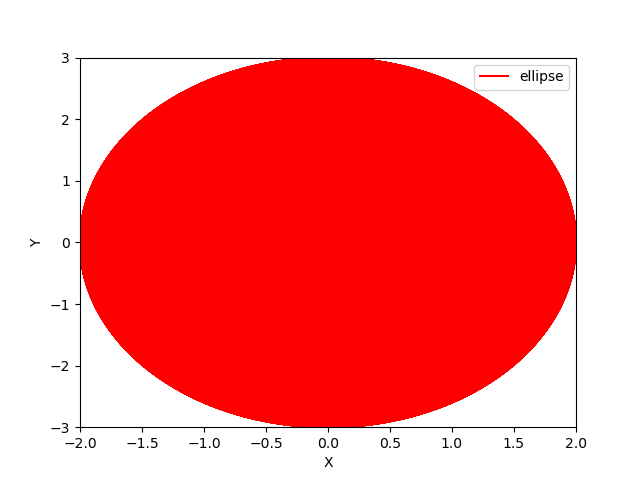
\includegraphics[width=0.7\columnwidth]{figs/fig.png}
    \caption{Approximate solution of the DE}
\end{figure}
\end{document}  
